\documentclass{beamer}
\usepackage[utf8]{inputenc}
\usepackage[french]{babel}
\usepackage[T1]{fontenc}
\usepackage{graphicx}
\usepackage{url}
\usepackage{alltt}

\usepackage{xcolor}
\definecolor{lightgreen}{rgb}{0.56, 0.93, 0.56}
\definecolor{blizzardblue}{rgb}{0.67, 0.9, 0.93}
\definecolor{lightgrey}{rgb}{0.7, 0.7, 0.7}
\definecolor{ansigreen}{rgb}{0.01, 0.75, 0.24}
\definecolor{ansired}{rgb}{0.79, 0.0, 0.09}
\definecolor{ansicyan}{rgb}{0.0, 0.77, 0.77}
\definecolor{ansiblue}{rgb}{0.08, 0.38, 0.74}

\usepackage{tikz}
\usetikzlibrary{shapes,shapes.geometric,shapes.symbols,arrows,shapes.multipart,positioning,calc,backgrounds,fit}

\tikzstyle{arrow} = [draw, latex-]
\tikzstyle{myrect} = [draw, rectangle, rounded corners=4pt, minimum width=16mm, minimum height=8mm]
\tikzstyle{commit} = [myrect, fill=lightgreen]
\tikzstyle{branch} = [myrect, fill=blizzardblue]
\tikzstyle{head} = [myrect, fill=lightgrey]

%\usetheme{Copenhagen}
\usecolortheme{beaver}

\setbeamertemplate{navigation symbols}{}

\DeclareGraphicsExtensions{.pdf,.png,.jpg}
\graphicspath{{./images/}}

\newcommand{\code}[1]{\texttt{#1}}
\newcommand{\opt}[1]{[-\hspace{0pt}-#1]}

\title[Git]{Git : un gestionnaire de versions intelligent}
\author{Benoit Daloze et Sébastien Wilmet}
\date{16 avril 2012}

\begin{document}

\usebackgroundtemplate{
\includegraphics[width=\paperwidth,height=\paperheight]{background}}
\begin{frame}
\titlepage
\begin{center}
  
\includegraphics[width=100pt]{git-logo}
\end{center}
\end{frame}

\usebackgroundtemplate{
\includegraphics[width=\paperwidth,height=\paperheight]{background-light}}

\begin{frame}
  \tableofcontents
\end{frame}

\section{Les gestionnaires de versions}
\begin{frame}
  \tableofcontents[sectionstyle=show/shaded]
\end{frame}

\usebackgroundtemplate{}

\begin{frame}{Moyens primitifs}
Gérer un projet de programmation sans gestionnaire de versions :
\begin{itemize}
  \item S'envoyer l'entièreté du code par mail ;
  \item Partage de fichiers sur un serveur (dropbox, …) ;
  \item S'envoyer des \textit{patchs} :
  \begin{itemize}
    \item commande \texttt{diff} : différence entre deux fichiers/dossiers ;
    \item commande \texttt{patch} : appliquer le \textit{patch} (la \textit{diff}).
  \end{itemize}
  \item etc.
\end{itemize}

\pause
\bigskip
Pas très pratique !
\end{frame}

\begin{frame}{Buts d'un gestionnaire de versions}
  \begin{itemize}
    \item Faciliter la gestion d'un projet de programmation ;
    \item Garder l'historique de toutes les modifications (\textit{commits}) ;
    \item Travailler en équipe ;
    \item Avoir des branches de développement :
      \begin{itemize}
        \item pour développer une fonctionnalité séparément ;
        \item pour une certaine version (2.4.0 $\rightarrow$ 2.4.1 $\rightarrow$ ...).
      \end{itemize}
  \end{itemize}

  \bigskip
  \begin{center}
    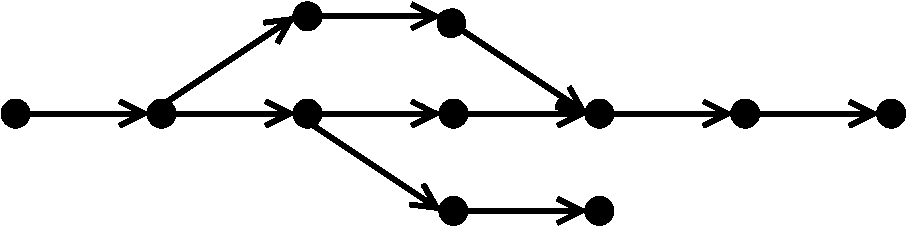
\includegraphics[scale=0.4]{commit-branch.pdf}
  \end{center}
\end{frame}

\begin{frame}{Micro-commits}
  Un \textit{commit} = \textbf{une} modification bien particulière

  \bigskip
  Avantages :
  \begin{itemize}
    \item Plus facile à comprendre pour les autres
    \item Possibilité d'annuler un changement facilement (\texttt{git revert})
    \item Trouver l'origine d'un bug (\texttt{git bisect})
    \item …
  \end{itemize}
\end{frame}

% He who controls the version control, controls the past.

\begin{frame}{Historique des gestionnaires de versions}
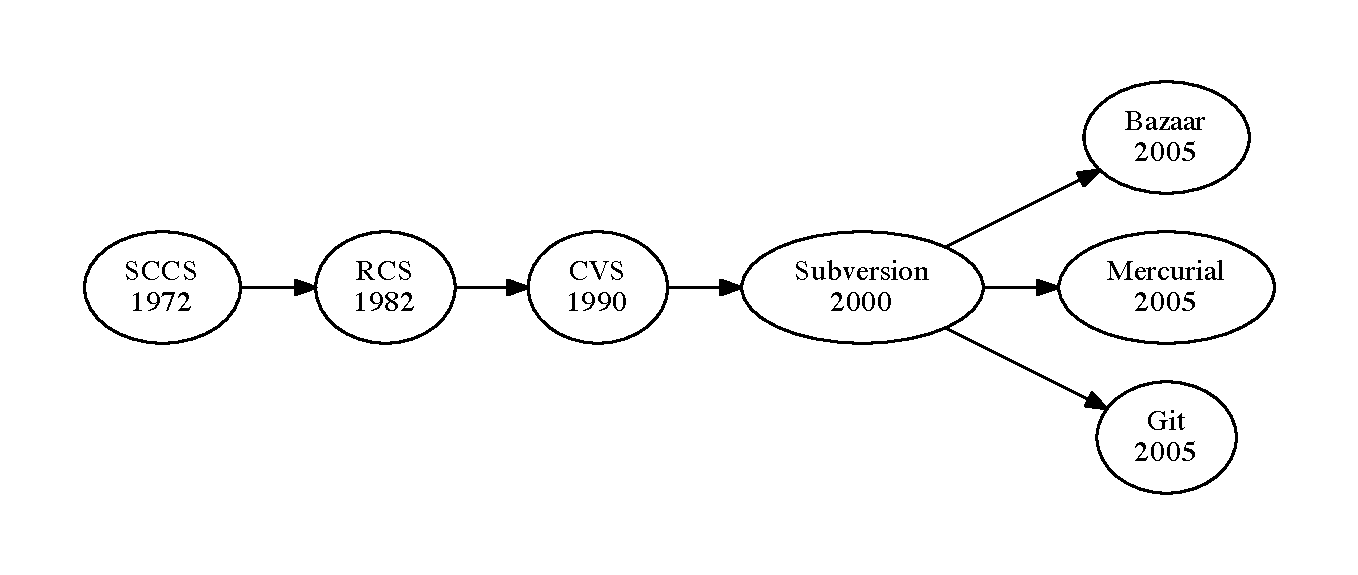
\includegraphics[width=\textwidth]{vcs-history.pdf}
\end{frame}

\begin{frame}{Subversion}
  Subversion (SVN) est \textbf{centralisé} :
  \begin{itemize}
    \item Un serveur central contient toutes les données ;
    \item Beaucoup de requêtes entre le client et le serveur (assez lent) ;
    \item Besoin d'une connexion internet pour travailler.
  \end{itemize}
\end{frame}

\begin{frame}{Git}
  Git est \textbf{décentralisé}/\textbf{distribué} :
  \begin{itemize}
    \item Toutes les données sont sur notre machine ;
    \item Les opérations sont très rapides ;
    \item Connexion internet seulement pour les \textit{pull} et \textit{push}.
  \end{itemize}

  \pause
  \bigskip
  Git est aussi \textbf{plus puissant} et \textbf{plus flexible} :
  \begin{itemize}
    \item Pour la gestion des branches ;
    \item Possède de nombreuses fonctionnalités plus avancées.
  \end{itemize}
\end{frame}

\begin{frame}{Serveur central avec Git}
  \begin{itemize}
    \item Une manière simple de travailler en équipe ;
    \item Accès en écriture pour tous les développeurs.
  \end{itemize}

  \bigskip
  \begin{center}
    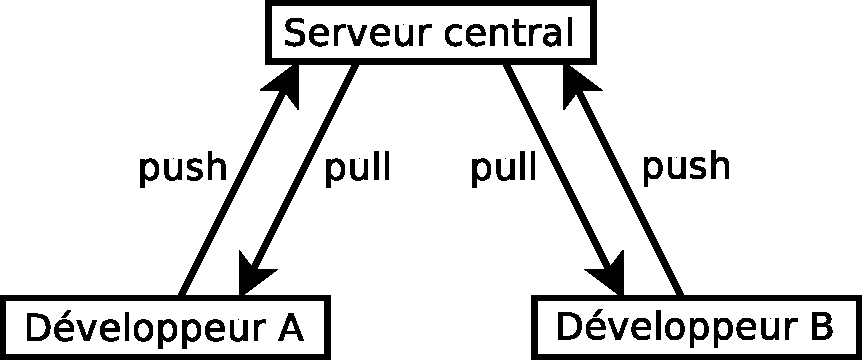
\includegraphics[scale=0.5]{pull-push-central-server.pdf}
  \end{center}
\end{frame}

\begin{frame}{Git est décentralisé}
  \begin{itemize}
    \item Seul les mainteneurs ont accès en écriture ;
    \item Les contributeurs font des \textit{pull requests}.
  \end{itemize}

  \bigskip
  \begin{center}
    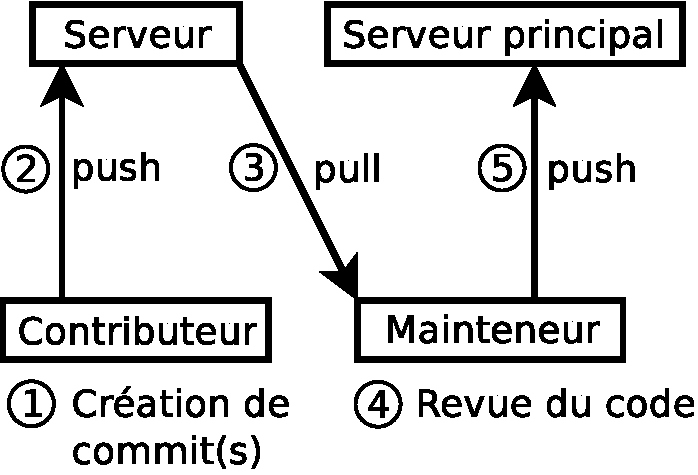
\includegraphics[scale=0.5]{pull-push-distributed.pdf}
  \end{center}
\end{frame}

\section{Commandes de base, créer un commit}

\usebackgroundtemplate{
\includegraphics[width=\paperwidth,height=\paperheight]{background-light}}
\begin{frame}
  \tableofcontents[sectionstyle=show/shaded]
\end{frame}
\usebackgroundtemplate{}

\begin{frame}[fragile]{Créer le dépôt Git}
  Pour un nouveau projet :
\begin{footnotesize}
\begin{verbatim}
$ mkdir project
$ cd project/
$ git init
\end{verbatim}
\end{footnotesize}

  \pause
  \bigskip
  Pour un projet existant :
\begin{footnotesize}
\begin{verbatim}
$ git clone git://example.net/project
$ cd project/
\end{verbatim}
\end{footnotesize}

  \pause
  \bigskip
  Répertoire caché \texttt{.git/} (unique) :
\begin{footnotesize}
\begin{verbatim}
$ ls .git/
config  description  HEAD  hooks/  info/  objects/  refs/
\end{verbatim}
\end{footnotesize}
\end{frame}

\begin{frame}{États d'un fichier}
  \textit{\textbf{Untracked}}
  \begin{itemize}
    \item non pris en compte par Git
  \end{itemize}

  \pause
  \medskip
  \textit{\textbf{Unmodified/Committed}}
  \begin{itemize}
    \item aucune modification
  \end{itemize}

  \pause
  \medskip
  \textit{\textbf{Modified}}
  \begin{itemize}
    \item fichier modifié
    \item pas pris en compte pour le prochain commit
  \end{itemize}

  \pause
  \medskip
  \textit{\textbf{Staged}}
  \begin{itemize}
    \item fichier ajouté, modifié, supprimé ou déplacé
    \item pris en compte pour le prochain commit
  \end{itemize}
\end{frame}

\begin{frame}{États d'un fichier}
\begin{center}
\begin{tikzpicture}[thick, node distance=40mm]
  \node [myrect] (wd) {Working directory};
  \node [myrect, below=10mm of wd, align=center, fill=red] (uu) {Untracked \\ Modified};
  \node [myrect, right of=wd] (staging) {Staging area};
  \node [myrect, right of=uu, align=center, fill=green] (staged) {Staged};
  \node [myrect, right of=staging] (repository) {Repository};
  \node [myrect, right of=staged, fill=yellow] (committed) {Committed};
  \draw [arrow] (staged) -- (uu) node [above,midway] {git add};
  \draw [arrow] (committed) -- (staged) node [above,midway] {git commit};
\end{tikzpicture}
\end{center}
\end{frame}

\begin{frame}[fragile]{Créer un nouveau fichier}
\begin{footnotesize}
\begin{verbatim}
$ echo hello > README
\end{verbatim}
\end{footnotesize}

État du fichier : \textit{\textbf{untracked}}

\pause
\begin{footnotesize}
\begin{alltt}
$ git status
# On branch master
#
# Initial commit
#
# \textcolor{ansired}{Untracked files}:
#   (use "git add <file>..." to include in what will be committed)
#
#       \textcolor{ansired}{README}
nothing added to commit but untracked files present
\end{alltt}
\end{footnotesize}
\end{frame}

\begin{frame}[fragile]{Créer un nouveau fichier}
\begin{footnotesize}
\begin{verbatim}
$ git add README
\end{verbatim}
\end{footnotesize}

État du fichier : \textit{\textbf{untracked}} $ \longrightarrow $ \textit{\textbf{staged}}

\pause
\begin{footnotesize}
\begin{alltt}
$ git status
# On branch master
#
# Initial commit
#
# Changes to be committed:
#   (use "git rm --cached <file>..." to unstage)
#
#	      \textcolor{ansigreen}{new file:   README}
#
\end{alltt}
\end{footnotesize}
\end{frame}

\begin{frame}[fragile]{Créer le commit}
\begin{footnotesize}
\begin{verbatim}
$ git commit
[écrire le message du commit]
\end{verbatim}

\pause
\begin{verbatim}
$ git log
commit c3aab8bb6cca644162a4fa82df283682717da3d4
Author: Your Name <foo@bar.be>
Date:   Wed Feb 1 15:19:03 2012 +0100

    Titre du commit (pas trop long)

    Plus longue description.
    Ligne vide après le titre.
\end{verbatim}
\end{footnotesize}
\end{frame}

\begin{frame}[fragile]{Modifier un fichier}
État du fichier README : \textit{\textbf{unmodified}}

\pause
\begin{footnotesize}
\begin{verbatim}
$ echo world >> README
\end{verbatim}
\end{footnotesize}

État : \textit{\textbf{modified}}

\pause
\begin{footnotesize}
\begin{verbatim}
$ git add README
\end{verbatim}
\end{footnotesize}

État : \textit{\textbf{staged}}

\pause
\begin{footnotesize}
\begin{verbatim}
$ git commit
\end{verbatim}
\end{footnotesize}

État : \textit{\textbf{committed}}
\end{frame}

\begin{frame}[fragile]{Diff}
  Voir les modifications avant de créer un commit.
\begin{small}
\begin{alltt}
$ echo new-text > README

$ git diff
diff --git a/README b/README
index 2e85c45..4320c6f 100644
--- a/README
+++ b/README
\textcolor{ansicyan}{@@ -1,2 +1 @@}
\textcolor{ansired}{-hello
-world}
\textcolor{ansigreen}{+new-text}
\end{alltt}
\end{small}
\end{frame}

\begin{frame}[fragile]{Aide}
La liste des commandes :
\begin{small}
\begin{verbatim}
$ git help
\end{verbatim}
\end{small}

\bigskip
Page de manuel d'une commande :
\begin{small}
\begin{verbatim}
$ git help <cmd>
$ git help <cmd> --web
$ git <cmd> --help
\end{verbatim}
\end{small}
\end{frame}

\begin{frame}{Résumé des commandes}
  \begin{ttfamily}
    \begin{itemize}
      \item git init
      \item git clone
      \item git status
      \item git add <file>
      \item git rm/mv <file>
      \item git commit
      \item git log
      \item git diff
      \item git help
    \end{itemize}
  \end{ttfamily}
\end{frame}

\section{Gérer plusieurs branches}

\usebackgroundtemplate{
\includegraphics[width=\paperwidth,height=\paperheight]{background-light}}
\begin{frame}
  \tableofcontents[sectionstyle=show/shaded]
\end{frame}
\usebackgroundtemplate{}

\begin{frame}{Créer une branche}
  Une branche :
  \begin{itemize}
    \item Pointe vers un commit ;
    \item Le pointeur «~avance~» quand on crée un commit.
  \end{itemize}

  \medskip
  Un commit pointe vers son ou ses commit(s) parent(s).

  \bigskip
  Créons une branche :

\begin{center}
  \begin{tikzpicture}[thick, node distance=28mm]
    \node (command) at (2,1.5) {\code{\$ git branch testing}};
    \node [commit] (98ca9) {98ca9};
    \node [commit, right of=98ca9] (34ac2) {34ac2};
    \draw [arrow] (98ca9) -- (34ac2);
    \node [commit, right of=34ac2] (f30ab) {f30ab};
    \draw [arrow] (34ac2) -- (f30ab);
    \node [branch, above=8mm of f30ab] (master) {master};
    \draw [arrow] (f30ab) -- (master);
    \node [branch, below=8mm of f30ab] (testing) {testing};
    \draw [arrow] (f30ab) -- (testing);
  \end{tikzpicture}
\end{center}
\end{frame}

\begin{frame}{HEAD}
Le pointeur \code{HEAD} pointe vers la branche courante.

\begin{center}
  \begin{tikzpicture}[thick, node distance=28mm]
    \node [align=left] (command) at (2,2) {\code{\$ git branch}\\
                                            \code{* \textcolor{ansigreen}{master}}\\
                                            \quad\code{testing}};
    \node [commit] (98ca9) {98ca9};
    \node [commit, right of=98ca9] (34ac2) {34ac2};
    \draw [arrow] (98ca9) -- (34ac2);
    \node [commit, right of=34ac2] (f30ab) {f30ab};
    \draw [arrow] (34ac2) -- (f30ab);
    \node [branch, above=8mm of f30ab] (master) {master};
    \draw [arrow] (f30ab) -- (master);
    \node [branch, below=8mm of f30ab] (testing) {testing};
    \draw [arrow] (f30ab) -- (testing);
    \node [head, above=8mm of master] (head) {HEAD};
    \draw [arrow] (master) -- (head);
  \end{tikzpicture}
\end{center}
\end{frame}

\begin{frame}{Changer de branche}
\begin{center}
  \begin{tikzpicture}[thick, node distance=28mm]
    \node (command) at (2,1.5) {\code{\$ git checkout testing}};
    \node [commit] (98ca9) {98ca9};
    \node [commit, right of=98ca9] (34ac2) {34ac2};
    \draw [arrow] (98ca9) -- (34ac2);
    \node [commit, right of=34ac2] (f30ab) {f30ab};
    \draw [arrow] (34ac2) -- (f30ab);
    \node [branch, above=8mm of f30ab] (master) {master};
    \draw [arrow] (f30ab) -- (master);
    \node [branch, below=8mm of f30ab] (testing) {testing};
    \draw [arrow] (f30ab) -- (testing);
    \node [head, below=8mm of testing] (head) {HEAD};
    \draw [arrow] (testing) -- (head);
  \end{tikzpicture}
\end{center}
\end{frame}

\begin{frame}{Créer un commit sur testing}
\begin{center}
  \begin{tikzpicture}[thick, node distance=28mm]
    \node (command) at (2,1.5) {\code{\$ git commit ...}};
    \node [commit] (98ca9) {98ca9};
    \node [commit, right of=98ca9] (34ac2) {34ac2};
    \draw [arrow] (98ca9) -- (34ac2);
    \node [commit, right of=34ac2] (f30ab) {f30ab};
    \draw [arrow] (34ac2) -- (f30ab);
    \node [branch, above=8mm of f30ab] (master) {master};
    \draw [arrow] (f30ab) -- (master);
    \node [commit, right of=f30ab] (c2b9e) {c2b9e};
    \draw [arrow] (f30ab) -- (c2b9e);
    \node [branch, below=8mm of c2b9e] (testing) {testing};
    \draw [arrow] (c2b9e) -- (testing);
    \node [head, below=8mm of testing] (head) {HEAD};
    \draw [arrow] (testing) -- (head);
  \end{tikzpicture}
\end{center}
\end{frame}

\begin{frame}{Revenir sur master}
\begin{center}
  \begin{tikzpicture}[thick, node distance=28mm]
    \node (command) at (2,1.5) {\code{\$ git checkout master}};
    \node [commit] (98ca9) {98ca9};
    \node [commit, right of=98ca9] (34ac2) {34ac2};
    \draw [arrow] (98ca9) -- (34ac2);
    \node [commit, right of=34ac2] (f30ab) {f30ab};
    \draw [arrow] (34ac2) -- (f30ab);
    \node [branch, above=8mm of f30ab] (master) {master};
    \draw [arrow] (f30ab) -- (master);
    \node [commit, right of=f30ab] (c2b9e) {c2b9e};
    \draw [arrow] (f30ab) -- (c2b9e);
    \node [branch, below=8mm of c2b9e] (testing) {testing};
    \draw [arrow] (c2b9e) -- (testing);
    \node [head, above=8mm of master] (head) {HEAD};
    \draw [arrow] (master) -- (head);
  \end{tikzpicture}
\end{center}
\end{frame}

\begin{frame}{Créer un commit sur master}
\begin{center}
  \begin{tikzpicture}[thick, node distance=28mm]
    \node (command) at (2,1.5) {\code{\$ git commit ...}};
    \node [commit] (98ca9) {98ca9};
    \node [commit, right of=98ca9] (34ac2) {34ac2};
    \draw [arrow] (98ca9) -- (34ac2);
    \node [commit, right of=34ac2] (f30ab) {f30ab};
    \draw [arrow] (34ac2) -- (f30ab);
    \node [commit, right of=f30ab, yshift=1cm] (87ab2) {87ab2};
    \draw [arrow] (f30ab) -- (87ab2);
    \node [branch, above=6mm of 87ab2] (master) {master};
    \draw [arrow] (87ab2) -- (master);
    \node [commit, right of=f30ab, yshift=-1cm] (c2b9e) {c2b9e};
    \draw [arrow] (f30ab) -- (c2b9e);
    \node [branch, below=6mm of c2b9e] (testing) {testing};
    \draw [arrow] (c2b9e) -- (testing);
    \node [head, above=6mm of master] (head) {HEAD};
    \draw [arrow] (master) -- (head);
  \end{tikzpicture}
\end{center}
\end{frame}

\begin{frame}{Divergence}
\begin{center}
  \begin{tikzpicture}[thick, node distance=28mm]
    \node (start) {};
    \node [commit, right of=start, xshift=-5mm] (f30ab) {f30ab};
    \draw [arrow,dashed] (start) -- (f30ab);
    \node [commit, right of=f30ab, yshift=1cm] (87ab2) {87ab2};
    \draw [arrow] (f30ab) -- (87ab2);
    \node [branch, above=6mm of 87ab2] (master) {master};
    \draw [arrow] (87ab2) -- (master);
    \node [commit, right of=f30ab, yshift=-1cm] (c2b9e) {c2b9e};
    \draw [arrow] (f30ab) -- (c2b9e);
    \node [branch, below=6mm of c2b9e] (testing) {testing};
    \draw [arrow] (c2b9e) -- (testing);
    \node [head, above=6mm of master] (head) {HEAD};
    \draw [arrow] (master) -- (head);
  \end{tikzpicture}
\end{center}
\end{frame}

\begin{frame}{Merge}
\begin{center}
  \begin{tikzpicture}[thick, node distance=28mm]
    \node (command) at (2,2) {\code{\$ git merge testing}};
    \node (start) {};
    \node [commit, right of=start, xshift=-5mm] (f30ab) {f30ab};
    \draw [arrow,dashed] (start) -- (f30ab);
    \node [commit, right of=f30ab, yshift=1cm] (87ab2) {87ab2};
    \draw [arrow] (f30ab) -- (87ab2);
    \node [commit, right of=f30ab, yshift=-1cm] (c2b9e) {c2b9e};
    \draw [arrow] (f30ab) -- (c2b9e);
    \node [commit, right of=87ab2, yshift=-1cm, align=center] (cf1a5) {cf1a5 \\ Merge testing};
    \draw [arrow] (87ab2) -- (cf1a5);
    \draw [arrow] (c2b9e) -- (cf1a5);
    \node [branch, above=6mm of cf1a5] (master) {master};
    \draw [arrow] (cf1a5) -- (master);
    \node [branch, below=6mm of c2b9e] (testing) {testing};
    \draw [arrow] (c2b9e) -- (testing);
    \node [head, above=6mm of master] (head) {HEAD};
    \draw [arrow] (master) -- (head);
  \end{tikzpicture}
\end{center}
\end{frame}

\begin{frame}
\begin{center}
  \begin{tikzpicture}[thick, node distance=28mm]
    \node (start) {};
    \node [commit, right of=start, xshift=-5mm] (f30ab) {f30ab};
    \draw [arrow,dashed] (start) -- (f30ab);
    \node [commit, right of=f30ab, yshift=1cm] (87ab2) {87ab2};
    \draw [arrow] (f30ab) -- (87ab2);
    \node [branch, above=6mm of 87ab2] (master) {master};
    \draw [arrow] (87ab2) -- (master);
    \node [commit, right of=f30ab, yshift=-1cm] (c2b9e) {c2b9e};
    \draw [arrow] (f30ab) -- (c2b9e);
    \node [branch, below=6mm of c2b9e] (testing) {testing};
    \draw [arrow] (c2b9e) -- (testing);
    \node [head, below=6mm of testing] (head) {HEAD};
    \draw [arrow] (testing) -- (head);
  \end{tikzpicture}
\end{center}
\end{frame}

\begin{frame}{Rebase}
\begin{center}
  \begin{tikzpicture}[thick, node distance=28mm]
    \node (command) at (2,2) {\code{\$ git rebase master}};
    \node (start) {};
    \node [commit, right of=start, xshift=-5mm] (f30ab) {f30ab};
    \draw [arrow,dashed] (start) -- (f30ab);
    \node [commit, right of=f30ab] (87ab2) {87ab2};
    \draw [arrow] (f30ab) -- (87ab2);
    \node [commit, right of=f30ab, yshift=-2cm, dashed, opacity=.5] (c2b9e) {c2b9e};
    \draw [arrow,dashed,opacity=.5] (f30ab) -- (c2b9e);
    \node [commit, right of=87ab2] (a071e) {a071e};
    \draw [arrow] (87ab2) -- (a071e);
    \draw [arrow,dashed,opacity=.5] (c2b9e) -- (a071e);
    \node [branch, above=6mm of 87ab2] (master) {master};
    \draw [arrow] (87ab2) -- (master);
    \node [branch, below=6mm of a071e] (testing) {testing};
    \draw [arrow] (a071e) -- (testing);
    \node [head, below=6mm of testing] (head) {HEAD};
    \draw [arrow] (testing) -- (head);
  \end{tikzpicture}
\end{center}
\end{frame}

\begin{frame}[fragile]{Remotes}
  Remote : référence vers un dépôt distant.

\begin{alltt}
$ git remote -v
origin	git://git.kernel.org/pub/scm/git/git.git (fetch)
origin	git://git.kernel.org/pub/scm/git/git.git (push)

$ git branch -a
* \textcolor{ansigreen}{master}
  \textcolor{ansired}{remotes/origin/HEAD -> origin/master
  remotes/origin/man
  remotes/origin/master
  remotes/origin/next}
\end{alltt}
\end{frame}

\begin{frame}{\code{git pull [remote] [branch]}}
  \code{git pull origin master}
  \begin{itemize}
    \item git fetch origin
    \item git merge origin/master
  \end{itemize}

  \begin{center}
    \begin{tikzpicture}[thick, node distance=28mm]
      \node [align=center] (command) at (2,2.5) {\code{\$ git fetch origin}};
      \node (start) {};
      \node [commit, right of=start, xshift=-5mm] (f30ab) {f30ab};
      \draw [arrow,dashed] (start) -- (f30ab);
      \node [commit, right of=f30ab] (c2b9e) {c2b9e};
      \draw [arrow] (f30ab) -- (c2b9e);
      \node [commit, right of=c2b9e] (a071e) {a071e};
      \draw [arrow] (c2b9e) -- (a071e);

      \node [branch, below=6mm of f30ab, opacity=.5] (old_origin_master) {origin/master};
      \draw [arrow, opacity=.5] (f30ab) -- (old_origin_master);
      \node [branch, above=6mm of f30ab] (master) {master};
      \draw [arrow] (f30ab) -- (master);

      \node [branch, below=6mm of a071e] (origin_master) {origin/master};
      \draw [arrow] (a071e) -- (origin_master);
    \end{tikzpicture}
  \end{center}
\end{frame}

\begin{frame}{\code{git pull [remote] [branch]}}
  \code{git pull origin master}
  \begin{itemize}
    \item git fetch origin
    \item git merge origin/master
  \end{itemize}

  \begin{center}
    \begin{tikzpicture}[thick, node distance=28mm]
      \node (command) at (2.5,2.5) {\code{\$ git merge origin/master}};
      \node (start) {};
      \node [commit, right of=start, xshift=-5mm] (f30ab) {f30ab};
      \draw [arrow,dashed] (start) -- (f30ab);
      \node [commit, right of=f30ab] (c2b9e) {c2b9e};
      \draw [arrow] (f30ab) -- (c2b9e);
      \node [commit, right of=c2b9e] (a071e) {a071e};
      \draw [arrow] (c2b9e) -- (a071e);

      \node [branch, above=6mm of f30ab, opacity=.5] (old_master) {master};
      \draw [arrow, opacity=.5] (f30ab) -- (old_master);

      \node [branch, below=6mm of a071e] (origin_master) {origin/master};
      \draw [arrow] (a071e) -- (origin_master);

      \node [branch, above=6mm of a071e] (master) {master};
      \draw [arrow] (a071e) -- (master);
    \end{tikzpicture}
  \end{center}
\end{frame}

\begin{frame}{\code{git pull : merge}}
  \begin{center}
    \begin{tikzpicture}[thick, node distance=28mm]
      \node (command) at (1,2) {\code{\$ git merge origin/master}};
      \node (start) {};
      \node [commit, right of=start, xshift=-5mm] (f30ab) {f30ab};
      \draw [arrow,dashed] (start) -- (f30ab);
      \node [commit, right of=f30ab, yshift=-1cm] (87ab2) {87ab2};
      \draw [arrow] (f30ab) -- (87ab2);
      \node [commit, right of=f30ab, yshift=1cm] (c2b9e) {c2b9e};
      \draw [arrow] (f30ab) -- (c2b9e);
      \node [commit, right of=87ab2, yshift=1cm, align=center] (merge) {Merge};
      \draw [arrow] (87ab2) -- (merge);
      \draw [arrow] (c2b9e) -- (merge);

      \node [branch, above=6mm of c2b9e, opacity=.5] (old_master) {master};
      \draw [arrow, opacity=.5] (c2b9e) -- (old_master);
      \node [branch, below=6mm of 87ab2] (origin_master) {origin/master};
      \draw [arrow] (87ab2) -- (origin_master);
      \node [branch, above=6mm of merge] (master) {master};
      \draw [arrow] (merge) -- (master);
    \end{tikzpicture}
  \end{center}
\end{frame}

\begin{frame}{\code{git pull \code{-}-rebase}}
  \begin{center}
    \begin{tikzpicture}[thick, node distance=28mm]
      \node (command) at (1,2) {\code{\$ git rebase origin/master}};
      \node (start) {};
      \node [commit, right of=start, xshift=-5mm] (f30ab) {f30ab};
      \draw [arrow,dashed] (start) -- (f30ab);
      \node [commit, right of=f30ab] (87ab2) {87ab2};
      \draw [arrow] (f30ab) -- (87ab2);
      \node [commit, right of=f30ab, yshift=2cm, dashed, opacity=.5] (c2b9e) {c2b9e};
      \node [commit, right of=87ab2] (a071e) {a071e};
      \draw [arrow] (87ab2) -- (a071e);
      \draw [arrow,dashed,opacity=.5] (f30ab) -- (c2b9e);
      \draw [arrow,dashed,opacity=.5] (c2b9e) -- (a071e);

      \node [branch, above=6mm of c2b9e,opacity=.5] (old_master) {master};
      \draw [arrow,opacity=.5] (c2b9e) -- (old_master);
      \node [branch, below=6mm of 87ab2] (origin_master) {origin/master};
      \draw [arrow] (87ab2) -- (origin_master);
      \node [branch, above=6mm of a071e] (master) {master};
      \draw [arrow] (a071e) -- (master);
    \end{tikzpicture}
  \end{center}
\end{frame}

\begin{frame}{\code{git push [remote] [branch]}}
  \begin{center}
    \begin{tikzpicture}[thick, node distance=28mm]
      \node (command) at (2.5,2.5) {\code{\$ git push origin master}};
      \node (start) {};
      \node [commit, right of=start, xshift=-5mm] (f30ab) {f30ab};
      \draw [arrow,dashed] (start) -- (f30ab);
      \node [commit, right of=f30ab] (c2b9e) {c2b9e};
      \draw [arrow] (f30ab) -- (c2b9e);
      \node [commit, right of=c2b9e] (a071e) {a071e};
      \draw [arrow] (c2b9e) -- (a071e);

      \node [branch, below=6mm of f30ab, opacity=.5] (old_origin_master) {origin/master};
      \draw [arrow, opacity=.5] (f30ab) -- (old_origin_master);

      \node [branch, below=6mm of a071e] (origin_master) {origin/master};
      \draw [arrow] (a071e) -- (origin_master);

      \node [branch, above=6mm of a071e] (master) {master};
      \draw [arrow] (a071e) -- (master);
    \end{tikzpicture}
  \end{center}
\end{frame}

\begin{frame}{Commandes principales}

\emph{browse} \begin{itemize}
  \item \code{git status}
  \item \code{git log}
  \item \code{git diff}
\end{itemize}

\emph{commit} \begin{itemize}
  \item \code{git add}
  \item \code{git commit}
\end{itemize}

\emph{branch} \begin{itemize}
  \item \code{git branch / checkout}
  \item \code{git merge / rebase}
\end{itemize}

\emph{remote} \begin{itemize}
  \item \code{git pull}
  \item \code{git push}
\end{itemize}

\end{frame}

\section{Autres fonctionnalités}

\usebackgroundtemplate{
\includegraphics[width=\paperwidth,height=\paperheight]{background-light}}
\begin{frame}
  \tableofcontents[sectionstyle=show/shaded]
\end{frame}
\usebackgroundtemplate{}

\begin{frame}{\code{git stash}}
\begin{center}
\begin{tikzpicture}[thick,commit2/.style={commit, node distance=11mm}]
  \node [commit2] (98ca9) {98ca9};
  \node [commit2, above of=98ca9] (34ac2) {34ac2};
  \draw [arrow] (98ca9) -- (34ac2);
  \node [commit2, above of=34ac2] (f30ab) {f30ab};
  \draw [arrow] (34ac2) -- (f30ab);
  \node [commit2, above of=f30ab] (c2b9e) {c2b9e};
  \draw [arrow] (f30ab) -- (c2b9e);
  \node [commit2, above of=c2b9e] (a071e) {a071e};
  \draw [arrow] (c2b9e) -- (a071e);

  \node [commit, right=25mm of c2b9e] (stash0) {stash@\{0\}};
  \node [commit, below of=stash0] (stash1) {stash@\{1\}};
  \node [commit, below of=stash1] (stash2) {stash@\{2\}};
  \node [commit, below of=stash2] (stash3) {...};
  \begin{pgfonlayer}{background}
    \node [head, fit=(stash0) (stash3)] {};
  \end{pgfonlayer}

  \draw [arrow, dashed, opacity=.5] (c2b9e) -- (stash0);
  \draw [arrow, dashed, opacity=.5] (c2b9e) -- (stash1);
  \draw [arrow, dashed, opacity=.5] (98ca9) -- (stash2);
\end{tikzpicture}
\end{center}
\end{frame}

\begin{frame}{\code{git stash}}
  git stash \begin{itemize}
    \item save [message]
    \pause
    \item list
    \item show [stash]
    \pause
    \item apply [stash]
    \item pop [stash]
  \end{itemize}
\end{frame}

\begin{frame}[fragile]{\code{git stash save}}
\begin{small}
\begin{alltt}
$ git status
# On branch master
# Changes not staged for commit:
#
#       \textcolor{ansired}{modified:   main.c}
#
no changes added to commit (use "git add"/"git commit -a")

$ git stash save
Saved working directory and index state WIP on master: 8540fea
HEAD is now at 8540fea message

$ git status
# On branch master
nothing to commit (working directory clean)
\end{alltt}
\end{small}
\end{frame}

\begin{frame}[fragile]{\code{git stash list, show}}
\begin{alltt}
$ git stash list
stash@\{0\}: WIP on master: 8540fea message

$ git stash show -p
\textcolor{ansired}{diff –git a/main.c b/main.c
index f2ad6c7..2f773ae 100644
--- a/main.c
+++ b/main.c}
\textcolor{ansicyan}{@@ -1,3 +1,5 @@}
\textcolor{ansigreen}{+#include <stdio.h>
+}
 int main() \{
    printf("Hello, world!");
    return 0;
 \}
\end{alltt}
\end{frame}

\begin{frame}{Commandes avancées}
  \textbf{git grep}
  \begin{itemize}
    \item grep(1) sur les fichiers pris en compte par git
  \end{itemize}

  \bigskip
  \textbf{git tag}
  \begin{itemize}
    \item crée un \emph{tag}, une référence fixe vers un commit
  \end{itemize}

  \bigskip
  \textbf{git revert}
  \begin{itemize}
    \item crée un \emph{commit} qui annule un autre
  \end{itemize}
\end{frame}

\begin{frame}[fragile]{\code{git blame}}
montre qui a modifié le fichier, ligne par ligne

\begin{footnotesize}
\begin{verbatim}
$ git blame git.c
85023 (Junio C Hamano      2006-12-19  1) #include "builtin.h"
2b11e (Johannes Schindelin 2006-06-05  2) #include "cache.h"
fd5c3 (Thiago Farina       2010-08-31  3) #include "exec_cmd.h"
fd5c3 (Thiago Farina       2010-08-31  4) #include "help.h"
575ba (Matthias Lederhofer 2006-06-25  5) #include "quote.h"
d8e96 (Jeff King           2009-01-28  6) #include "run-command.h"
8e49d (Andreas Ericsson    2005-11-16  7)
822a7 (Ramsay Allan Jones  2006-07-30  8) const char git_usage_string[] =
f2dd8 (Jon Seymour         2011-05-01  9)        "git [--version] [--exec-path[=<path>]] [--html-path] [--man-path] [--info-path]\n"
\end{verbatim}
\end{footnotesize}
\end{frame}

\begin{frame}[fragile]{\code{git reset}}
Change le pointeur de la branche courante
\begin{footnotesize}
\begin{alltt}
$ git reset HEAD^ # recule la branche d'un commit
Unstaged changes after reset:
M      README

$ git status
# On branch master
# Changes not staged for commit:
#
#       \textcolor{ansired}{modified:   README}
\end{alltt}
\begin{center}
\begin{tikzpicture}[thick, node distance=25mm]
  \node [align=center] (command) at (2,2.3) {\code{\$ git reset \code{-}-hard 98ca9}};
  \node [commit] (98ca9) {98ca9};
  \node [commit, right of=98ca9] (34ac2) {34ac2};
  \draw [arrow] (98ca9) -- (34ac2);
  \node [commit, right of=34ac2] (f30ab) {f30ab};
  \draw [arrow] (34ac2) -- (f30ab);

  \node [branch, above=6mm of f30ab, opacity=.5] (old_master) {master};
  \draw [arrow, opacity=.5] (f30ab) -- (old_master);

  \node [branch, above=6mm of 98ca9] (master) {master};
  \draw [arrow] (98ca9) -- (master);
\end{tikzpicture}
\end{center}
\end{footnotesize}
\end{frame}

\begin{frame}[fragile]{\code{git commit \code{-}-amend}}
Pour modifier le dernier \emph{commit} :
\begin{itemize}
  \item ajouter une modification ;
  \item modifier le message du \emph{commit}.
\end{itemize}

\bigskip
\begin{verbatim}
$ edit some_file
$ git add some_file
$ git commit --amend
\end{verbatim}
\end{frame}

\begin{frame}[fragile]{\code{git rebase \code{-}-interactive}}
Permet de modifier l'historique
\begin{footnotesize}
\begin{verbatim}
$ git rebase -i HEAD~3

pick 4eeebe5 bulk-checkin: allow the same data to be multiply hashed
pick 127b177 bulk-checkin: support chunked-object encoding
pick 973951a chunked-object: fallback checkout codepaths

# Rebase 617312b..973951a onto 617312b
#
# Commands:
#  p, pick = use commit
#  r, reword = use commit, but edit the commit message
#  e, edit = use commit, but stop for amending
#  s, squash = use commit, but meld into previous commit
#  f, fixup = like "squash", but discard this commit's log message
#  x, exec = run command (the rest of the line) using shell
#
# If you remove a line here THAT COMMIT WILL BE LOST.
# However, if you remove everything, the rebase will be aborted.
#
\end{verbatim}
\end{footnotesize}
\end{frame}

\begin{frame}[fragile]{\code{git reflog}}
Log des opérations sur les \emph{commits}
\begin{footnotesize}
\begin{verbatim}
$ git reflog
b0d66 HEAD@{0}: commit (amend): add a setting to require a filter to be successful
97395 HEAD@{1}: checkout: moving from master to man
b0d66 HEAD@{2}: rebase: aborting
9cda8 HEAD@{3}: rebase -i (pick): grep: drop grep_buffer's "name" parameter
b9ef9 HEAD@{4}: rebase -i (pick): convert git-grep to use grep_source interface
837de HEAD@{5}: rebase -i (pick): grep: make locking flag global
84f3d HEAD@{6}: checkout: moving from master to 84f3d
b0d66 HEAD@{7}: pull: Fast-forward
f6b50 HEAD@{8}: cherry-pick: add a TODO
98c05 HEAD@{9}: reset: moving to HEAD^
e11ee HEAD@{10}: checkout: moving from master to pu
77eac HEAD@{11}: commit: add a TODO
75f43 HEAD@{12}: commit: use the correct format identifier for unsigned long: %lu
f88cc HEAD@{13}: pull --rebase: git grep
07873 HEAD@{14}: pull : Fast-forward
f70f7 HEAD@{15}: clone: from git://git.kernel.org/pub/scm/git/git.git
\end{verbatim}
\end{footnotesize}
\end{frame}

\begin{frame}[fragile]{\code{git add \code{-}-patch}}
Permet d'ajouter une partie des modifications d'un fichier
\begin{footnotesize}
\begin{alltt}
$ git add -p
diff --git a/README b/README
\textcolor{ansicyan}{@@ -1,5 +1,7 @@}
 1
\textcolor{ansigreen}{+2}
 3
\textcolor{ansigreen}{+4}
\textcolor{ansiblue}{Stage this hunk [y,n,q,a,d,/,s,e,?]?} s
Split into 2 hunks.
\textcolor{ansicyan}{@@ -1,2 +1,3 @@}
 1
\textcolor{ansigreen}{+2}
 3
\textcolor{ansiblue}{Stage this hunk [y,n,q,a,d,/,j,J,g,e,?]?} n
\textcolor{ansicyan}{@@ -2,4 +3,5 @@}
 3
\textcolor{ansigreen}{+4}
\textcolor{ansiblue}{Stage this hunk [y,n,q,a,d,/,K,g,e,?]?} y
\end{alltt}
\end{footnotesize}
\end{frame}

\begin{frame}{git cherry-pick}
Applique un \emph{commit} sur la branche courante.

\begin{center}
\begin{tikzpicture}[thick, node distance=25mm]
  \node [align=center] (command) at (2,2.5) {\code{\$ git cherry-pick 4ce4a}};
  \node [commit] (98ca9) {98ca9};
  \node [commit, right of=98ca9] (34ac2) {34ac2};
  \draw [arrow] (98ca9) -- (34ac2);
  \node [commit, right of=34ac2] (f30ab) {f30ab};
  \draw [arrow] (34ac2) -- (f30ab);

  \node [commit, below=8mm of 98ca9] (bf7e0) {bf7e0};
  \node [commit, right of=bf7e0] (4ce4a) {4ce4a};
  \draw [arrow] (bf7e0) -- (4ce4a);
  \node [commit, right of=4ce4a] (e73f0) {e73f0};
  \draw [arrow] (4ce4a) -- (e73f0);
  \node [commit, right of=e73f0] (ffbcb) {ffbcb};
  \draw [arrow] (e73f0) -- (ffbcb);

  \node [branch, above=6mm of 34ac2, opacity=.5] (old_master) {master};
  \draw [arrow, opacity=.5] (34ac2) -- (old_master);

  \node [branch, above=6mm of f30ab] (master) {master};
  \draw [arrow] (f30ab) -- (master);

  \node [branch, below=6mm of ffbcb] (feature) {feature};
  \draw [arrow] (ffbcb) -- (feature);

  \draw [arrow, dashed, opacity=.5] (f30ab) -- (4ce4a);
\end{tikzpicture}
\end{center}
\end{frame}

\begin{frame}[fragile]{\code{git bisect}}
Permet de trouver l'origine d'un bug

\begin{footnotesize}
\begin{verbatim}
$ git bisect start bad_commit good_commit
Bisecting: 20 revisions left to test after this (roughly 4 steps)
[e4f3edc] Sync with maint

$ git bisect run ./mytests
Bisecting: 9 revisions left to test after this (roughly 3 steps)
[42226d] pack-objects: remove bogus comment
...
Bisecting: 0 revisions left to test after this (roughly 1 step)
[9a4749] checkout -m: no need to insist on having all 3 stages

8280f2e0a0f4776c4b3008c9172fc0a3e7361534 is the first bad commit
commit 8280f2e0a0f4776c4b3008c9172fc0a3e7361534
Author: eregon <mail@me>
Date:   Sat Feb 18 17:36:47 2012 +0100

    Noooo! You found my hidden bug!
\end{verbatim}
\end{footnotesize}
\end{frame}

% expain briefly internals: sha1, parents, ...

\begin{frame}{Services d'hébergement}
  \begin{itemize}
    \item GitHub
    \medskip
    \item Gitorious
    \medskip
    \item Bitbucket, assembla (dépôts privés gratuits)
    \medskip
    \item En INGI (voir le wiki)
          \url{http://wiki.student.info.ucl.ac.be/index.php/Git}
  \end{itemize}
\end{frame}

\usebackgroundtemplate{
\includegraphics[width=\paperwidth,height=\paperheight]{background-light}}
\begin{frame}{Liens}
\begin{itemize}
  \item Les manpages: \code{git help [-\code{-}web] <cmd>}
  \item \url{http://git-scm.com/book}: Pro Git book
  \item \url{http://louvilug.tuxfamily.org/}: Slides, aide-mémoire, exercices
\end{itemize}
\end{frame}
\usebackgroundtemplate{}


\end{document}
